% CVPR 2025 Paper Template; see https://github.com/cvpr-org/author-kit

\documentclass[10pt,twocolumn,letterpaper]{article}

%%%%%%%%% PAPER TYPE  - PLEASE UPDATE FOR FINAL VERSION
% \usepackage{cvpr}              % To produce the CAMERA-READY version
% \usepackage[review]{cvpr}      % To produce the REVIEW version
\usepackage[pagenumbers]{cvpr} % To force page numbers, e.g. for an arXiv version

% Import additional packages in the preamble file, before hyperref
%
% --- inline annotations
%
\newcommand{\red}[1]{{\color{red}#1}}
\newcommand{\todo}[1]{{\color{red}#1}}
\newcommand{\TODO}[1]{\textbf{\color{red}[TODO: #1]}}
% --- disable by uncommenting  
% \renewcommand{\TODO}[1]{}
% \renewcommand{\todo}[1]{#1}



% It is strongly recommended to use hyperref, especially for the review version.
% hyperref with option pagebackref eases the reviewers' job.
% Please disable hyperref *only* if you encounter grave issues, 
% e.g. with the file validation for the camera-ready version.
%
% If you comment hyperref and then uncomment it, you should delete *.aux before re-running LaTeX.
% (Or just hit 'q' on the first LaTeX run, let it finish, and you should be clear).
\definecolor{cvprblue}{rgb}{0.21,0.49,0.74}
\usepackage[pagebackref,breaklinks,colorlinks,allcolors=cvprblue]{hyperref}

%%%%%%%%% PAPER ID  - PLEASE UPDATE
\def\paperID{*****} % *** Enter the Paper ID here
\def\confName{CVPR}
\def\confYear{2025}

%%%%%%%%% TITLE - PLEASE UPDATE
\title{Enhancing Image Segmentation: A Comparative Study}

%%%%%%%%% AUTHORS - PLEASE UPDATE
\author{Aaryan,  \quad  Aayush Kumar, \quad  Darpan Gaur, \quad  Varun Gupta\\
Indian Institute of Technology Hyderabad\\
{\tt\small \{co21btech11001, co21btech11002, co21btech11004, cs21btech11060\}@iith.ac.in}
}

\begin{document}
\maketitle
\begin{abstract}
    Image segmentation is a crucial task in computer vision with significant applications in various fields such as autonomous driving, medical imaging, and object detection. Accurate segmentation allows for precise identification and localization of objects within an image, which is essential for tasks that require detailed scene understanding. In this project, we aim to compare the performance of different image segmentation models, including Convolutional Neural Networks (CNNs), Graph Convolutional Networks (GraphCNNs), and Transformers. Our goal is to evaluate their effectiveness and identify the strengths and weaknesses of each approach in the context of image segmentation. This literature survey was greatly inspired by \cite{9356353}.
\end{abstract}    
\section{Introduction}
\label{sec:intro}

Please follow the steps outlined below when submitting your manuscript to the IEEE Computer Society Press.
This style guide now has several important modifications (for example, you are no longer warned against the use of sticky tape to attach your artwork to the paper), so all authors should read this new version.

%-------------------------------------------------------------------------
\subsection{Language}

All manuscripts must be in English.

\subsection{Dual submission}

Please refer to the author guidelines on the \confName\ \confYear\ web page for a
discussion of the policy on dual submissions.

\subsection{Paper length}
Papers, excluding the references section, must be no longer than eight pages in length.
The references section will not be included in the page count, and there is no limit on the length of the references section.
For example, a paper of eight pages with two pages of references would have a total length of 10 pages.
{\bf There will be no extra page charges for \confName\ \confYear.}

Overlength papers will simply not be reviewed.
This includes papers where the margins and formatting are deemed to have been significantly altered from those laid down by this style guide.
Note that this \LaTeX\ guide already sets figure captions and references in a smaller font.
The reason such papers will not be reviewed is that there is no provision for supervised revisions of manuscripts.
The reviewing process cannot determine the suitability of the paper for presentation in eight pages if it is reviewed in eleven.

%-------------------------------------------------------------------------
\subsection{The ruler}
The \LaTeX\ style defines a printed ruler which should be present in the version submitted for review.
The ruler is provided in order that reviewers may comment on particular lines in the paper without circumlocution.
If you are preparing a document using a non-\LaTeX\ document preparation system, please arrange for an equivalent ruler to appear on the final output pages.
The presence or absence of the ruler should not change the appearance of any other content on the page.
The camera-ready copy should not contain a ruler.
(\LaTeX\ users may use options of \texttt{cvpr.sty} to switch between different versions.)

Reviewers:
note that the ruler measurements do not align well with lines in the paper --- this turns out to be very difficult to do well when the paper contains many figures and equations, and, when done, looks ugly.
Just use fractional references (\eg, this line is $087.5$), although in most cases one would expect that the approximate location will be adequate.


\subsection{Paper ID}
Make sure that the Paper ID from the submission system is visible in the version submitted for review (replacing the ``*****'' you see in this document).
If you are using the \LaTeX\ template, \textbf{make sure to update paper ID in the appropriate place in the tex file}.


\subsection{Mathematics}

Please number all of your sections and displayed equations as in these examples:
\begin{equation}
  E = m\cdot c^2
  \label{eq:important}
\end{equation}
and
\begin{equation}
  v = a\cdot t.
  \label{eq:also-important}
\end{equation}
It is important for readers to be able to refer to any particular equation.
Just because you did not refer to it in the text does not mean some future reader might not need to refer to it.
It is cumbersome to have to use circumlocutions like ``the equation second from the top of page 3 column 1''.
(Note that the ruler will not be present in the final copy, so is not an alternative to equation numbers).
All authors will benefit from reading Mermin's description of how to write mathematics:
\url{http://www.pamitc.org/documents/mermin.pdf}.

\subsection{Blind review}

Many authors misunderstand the concept of anonymizing for blind review.
Blind review does not mean that one must remove citations to one's own work---in fact it is often impossible to review a paper unless the previous citations are known and available.

Blind review means that you do not use the words ``my'' or ``our'' when citing previous work.
That is all.
(But see below for tech reports.)

Saying ``this builds on the work of Lucy Smith [1]'' does not say that you are Lucy Smith;
it says that you are building on her work.
If you are Smith and Jones, do not say ``as we show in [7]'', say ``as Smith and Jones show in [7]'' and at the end of the paper, include reference 7 as you would any other cited work.

An example of a bad paper just asking to be rejected:
\begin{quote}
\begin{center}
    An analysis of the frobnicatable foo filter.
\end{center}

   In this paper we present a performance analysis of our previous paper [1], and show it to be inferior to all previously known methods.
   Why the previous paper was accepted without this analysis is beyond me.

   [1] Removed for blind review
\end{quote}


An example of an acceptable paper:
\begin{quote}
\begin{center}
     An analysis of the frobnicatable foo filter.
\end{center}

   In this paper we present a performance analysis of the  paper of Smith \etal [1], and show it to be inferior to all previously known methods.
   Why the previous paper was accepted without this analysis is beyond me.

   [1] Smith, L and Jones, C. ``The frobnicatable foo filter, a fundamental contribution to human knowledge''. Nature 381(12), 1-213.
\end{quote}

If you are making a submission to another conference at the same time, which covers similar or overlapping material, you may need to refer to that submission in order to explain the differences, just as you would if you had previously published related work.
In such cases, include the anonymized parallel submission~\cite{Authors14} as supplemental material and cite it as
\begin{quote}
[1] Authors. ``The frobnicatable foo filter'', F\&G 2014 Submission ID 324, Supplied as supplemental material {\tt fg324.pdf}.
\end{quote}

Finally, you may feel you need to tell the reader that more details can be found elsewhere, and refer them to a technical report.
For conference submissions, the paper must stand on its own, and not {\em require} the reviewer to go to a tech report for further details.
Thus, you may say in the body of the paper ``further details may be found in~\cite{Authors14b}''.
Then submit the tech report as supplemental material.
Again, you may not assume the reviewers will read this material.

Sometimes your paper is about a problem which you tested using a tool that is widely known to be restricted to a single institution.
For example, let's say it's 1969, you have solved a key problem on the Apollo lander, and you believe that the 1970 audience would like to hear about your
solution.
The work is a development of your celebrated 1968 paper entitled ``Zero-g frobnication: How being the only people in the world with access to the Apollo lander source code makes us a wow at parties'', by Zeus \etal.

You can handle this paper like any other.
Do not write ``We show how to improve our previous work [Anonymous, 1968].
This time we tested the algorithm on a lunar lander [name of lander removed for blind review]''.
That would be silly, and would immediately identify the authors.
Instead write the following:
\begin{quotation}
\noindent
   We describe a system for zero-g frobnication.
   This system is new because it handles the following cases:
   A, B.  Previous systems [Zeus et al. 1968] did not  handle case B properly.
   Ours handles it by including a foo term in the bar integral.

   ...

   The proposed system was integrated with the Apollo lunar lander, and went all the way to the moon, don't you know.
   It displayed the following behaviours, which show how well we solved cases A and B: ...
\end{quotation}
As you can see, the above text follows standard scientific convention, reads better than the first version, and does not explicitly name you as the authors.
A reviewer might think it likely that the new paper was written by Zeus \etal, but cannot make any decision based on that guess.
He or she would have to be sure that no other authors could have been contracted to solve problem B.
\medskip

\noindent
FAQ\medskip\\
{\bf Q:} Are acknowledgements OK?\\
{\bf A:} No.  Leave them for the final copy.\medskip\\
{\bf Q:} How do I cite my results reported in open challenges?
{\bf A:} To conform with the double-blind review policy, you can report results of other challenge participants together with your results in your paper.
For your results, however, you should not identify yourself and should not mention your participation in the challenge.
Instead present your results referring to the method proposed in your paper and draw conclusions based on the experimental comparison to other results.\medskip\\

\begin{figure}[t]
  \centering
  \fbox{\rule{0pt}{2in} \rule{0.9\linewidth}{0pt}}
   %\includegraphics[width=0.8\linewidth]{egfigure.eps}

   \caption{Example of caption.
   It is set in Roman so that mathematics (always set in Roman: $B \sin A = A \sin B$) may be included without an ugly clash.}
   \label{fig:onecol}
\end{figure}

\subsection{Miscellaneous}

\noindent
Compare the following:\\
\begin{tabular}{ll}
 \verb'$conf_a$' &  $conf_a$ \\
 \verb'$\mathit{conf}_a$' & $\mathit{conf}_a$
\end{tabular}\\
See The \TeX book, p165.

The space after \eg, meaning ``for example'', should not be a sentence-ending space.
So \eg is correct, {\em e.g.} is not.
The provided \verb'\eg' macro takes care of this.

When citing a multi-author paper, you may save space by using ``et alia'', shortened to ``\etal'' (not ``{\em et.\ al.}'' as ``{\em et}'' is a complete word).
If you use the \verb'\etal' macro provided, then you need not worry about double periods when used at the end of a sentence as in Alpher \etal.
However, use it only when there are three or more authors.
Thus, the following is correct:
   ``Frobnication has been trendy lately.
   It was introduced by Alpher~\cite{Alpher02}, and subsequently developed by
   Alpher and Fotheringham-Smythe~\cite{Alpher03}, and Alpher \etal~\cite{Alpher04}.''

This is incorrect: ``... subsequently developed by Alpher \etal~\cite{Alpher03} ...'' because reference~\cite{Alpher03} has just two authors.

\begin{figure*}
  \centering
  \begin{subfigure}{0.68\linewidth}
    \fbox{\rule{0pt}{2in} \rule{.9\linewidth}{0pt}}
    \caption{An example of a subfigure.}
    \label{fig:short-a}
  \end{subfigure}
  \hfill
  \begin{subfigure}{0.28\linewidth}
    \fbox{\rule{0pt}{2in} \rule{.9\linewidth}{0pt}}
    \caption{Another example of a subfigure.}
    \label{fig:short-b}
  \end{subfigure}
  \caption{Example of a short caption, which should be centered.}
  \label{fig:short}
\end{figure*}

\section{Literature Review}
\label{sec:literature}

\subsection{Convolutional Neural Network Architectures}
Convolutional Neural Networks (CNNs) have been a fundamental approach in the field of image processing, particularly in the domain of image segmentation. This section reviews three prominent CNN architectures: Fully Convolutional Networks (FCN), UNet++, and DeepLabV3+, highlighting their innovations, strengths, weaknesses, and typical use cases.

\subsubsection{Fully Convolutional Networks (FCN)}
Introduced by \textit{Long et al.} in 2015, the key innovation of FCN is its fully convolutional nature, which allows it to operate on input images of any size \cite{long2015fcn}. This architecture is simple and flexible, attributed to its use of convolutional layers that replace fully connected layers, enabling the network to efficiently learn spatial hierarchies for pixel-wise segmentation.

\noindent \textbf{Strengths:}
\begin{itemize}
  \item Simple and flexible architecture.
  \item Efficient in learning spatial hierarchies.
\end{itemize}

\noindent \textbf{Weaknesses:}
\begin{itemize}
  \item Produces coarse segmentation maps, lacking in fine detail.
\end{itemize}

\noindent \textbf{Best Use Case:}
\begin{itemize}
  \item General segmentation tasks where detailed precision is less critical.
\end{itemize}

\subsubsection{UNet++}
UNet++ is a more advanced variant that introduces nested dense skip connections to improve the fine-grained segmentation capability, particularly beneficial in medical imaging \cite{zhou2019unet++}. The architecture includes several enhancements such as deep supervision and feature fusion, which allow for more precise and detailed segmentation outputs.

\noindent \textbf{Key Features:}
\begin{itemize}
  \item Nested skip connections facilitate feature refinement across different network layers.
  \item Deep supervision at multiple decoder levels enhances the training dynamics.
  \item Feature fusion through decoder nodes integrates information from multiple preceding layers.
\end{itemize}

\noindent \textbf{Advantages:}
\begin{itemize}
  \item Achieves fine-grained segmentation, crucial for medical applications.
  \item Manages computational costs effectively compared to more complex models.
\end{itemize}

\noindent \textbf{Weakness:}
\begin{itemize}
  \item Slightly higher computational overhead than basic UNet due to additional connections.
\end{itemize}

\noindent \textbf{Best Use Case:}
\begin{itemize}
  \item High-resolution medical image segmentation where detail is paramount.
\end{itemize}

\subsubsection{DeepLabV3+}
DeepLabV3+, developed by \textit{Chen et al.}, incorporates atrous convolution and an atrous spatial pyramid pooling (ASPP) module to effectively capture multi-scale contextual information \cite{chen2018deeplabv3+}. This design allows the network to handle complex scenes with varying object scales efficiently.

\noindent \textbf{Strengths:}
\begin{itemize}
  \item Handles multiple scales effectively using ASPP.
  \item Suitable for complex scene segmentation with high variability in object size and structure.
\end{itemize}

\noindent \textbf{Weaknesses:}
\begin{itemize}
  \item Computationally intensive, requiring significant resources.
\end{itemize}

\noindent \textbf{Best Use Case:}
\begin{itemize}
  \item Complex scene segmentation such as urban landscapes or densely populated images.
\end{itemize}

\subsection{UNet++}
UNet++ is an enhanced structure of the traditional UNet model designed to achieve more accurate segmentation, especially in medical imaging applications. It introduces several innovative concepts:

\paragraph{Nested Skip Connections}
These connections are comprised of multiple intermediate nodes that refine and combine features from various network paths, enhancing the network's ability to propagate context and capture detailed structures within the image.

\paragraph{Deep Supervision}
UNet++ incorporates output layers attached at multiple decoder levels, facilitating the direct influence of the loss function across different depths of the network. This approach helps in the faster convergence of the network and improves the gradient flow, leading to enhanced learning capabilities.

\paragraph{Feature Fusion}
The decoder nodes in UNet++ integrate information from both preceding layers and skip connections. This fusion occurs via up-sampling and convolutions, allowing the network to preserve essential details and improve the quality of the segmentation output.

\begin{figure}[h]
\centering
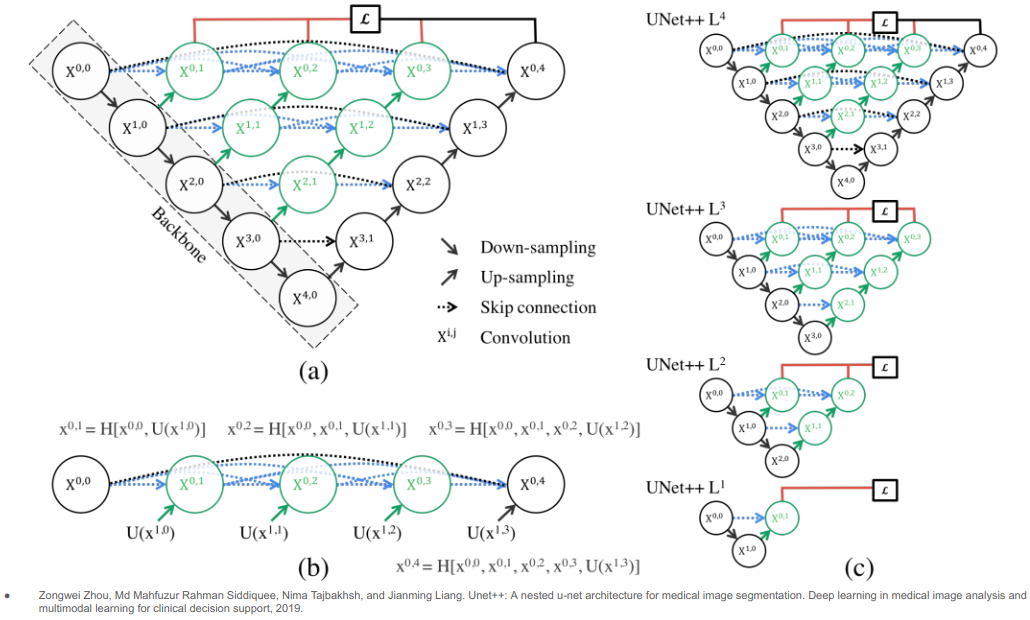
\includegraphics[width=0.48\textwidth]{images/unet_plus_architecture.png}
\caption{The architecture of UNet++ showing nested skip connections, deep supervision, and feature fusion mechanisms.}
\label{fig:unet_plus_architecture}
\end{figure}

\paragraph{Mathematical Formulation}
The operations within the UNet++ can be described by the following equation:
\[
F_{i,j} = H_{i,j} \left( F_{i-1,j} + \sum_{k=0}^{j-1} H_{i,k} \right)
\]
where \( F_{i,j} \) represents the feature map at the \( j^{th} \) node of the \( i^{th} \) layer, \( H_{i,j} \) is the convolution operation at node \( j \) of layer \( i \), and the summation aggregates the feature maps from all previous nodes at the same layer, enhancing the feature integration across the network.

\paragraph{Advantages}
\begin{itemize}
    \item UNet++ is capable of capturing detailed features such as water boundaries, which is critical for applications like flood area segmentation.
    \item It performs well on smaller datasets, a common limitation in specialized fields such as medical imaging, where large annotated datasets may not be available.
    \item The computation cost, while higher than simpler architectures like FCN, remains manageable and less intensive compared to more complex models like DeepLabV3+.
\end{itemize}

\paragraph{Applications}
UNet++ is particularly suited for high-resolution image tasks where detailed feature delineation is critical. It has shown promising results in medical imaging, including tasks like tumor segmentation and organ delineation.

\subsection{Graph Neural Networks: Graph-FCN and CNN-G}

Deep learning has made significant advancements in semantic segmentation by classifying pixels in images. However, during high-level feature extraction, it often ignores the local spatial information, which is important for accurate segmentation. Graph-based models address this limitation by including the missing local context.

\subsubsection{Graph-FCN}

Graph-FCN combines graph convolutional networks (GCNs) with fully convolutional networks (FCNs) to capture local spatial relationships in images. Initially, a convolutional network converts the image grid data into a graph structure, transforming the semantic segmentation task into a graph node classification problem. The graph convolutional network is then applied to classify the nodes in this graph, effectively solving the segmentation challenge.

FCN-16s generates feature maps, and node annotations are initialized by combining upsampled feature vectors and node locations. Labels for nodes are obtained by pooling the raw label image during training. The process is shown in Figure~\ref{fig:graphfcn_node_init}.

\begin{figure}
    \centering
    % \fbox{\rule{0pt}{2in} \rule{0.9\linewidth}{0pt}}
    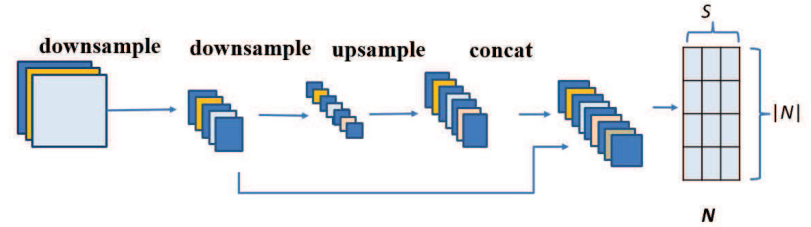
\includegraphics[width=0.8\linewidth]{images/graphfcn_node_init.png}
    \caption{Graph-FCN node initialization. From ~\cite{lu2020graphfcnimagesemanticsegmentation}.}
    \label{fig:graphfcn_node_init}
\end{figure}

In the graph model, edges are represented by an adjacency matrix, where each node is connected to its nearest $l$ nodes. These connections allow node annotations to transfer through the edges in the graph neural network.

FCN-16s handles node classification and graph model initialization on a small feature map, while a 2-layer GCN classifies the nodes within the graph. Cross-entropy loss is computed for both outputs, and like FCN-16s, Graph-FCN is trained end-to-end. The output of the prediction process is the output of the convolutional network. The graph model is only used during the training.

The structure of the Graph-FCN model is shown in Figure~\ref{fig:graphfcn_structure}.
\begin{figure}
    \centering
    % \fbox{\rule{0pt}{2in} \rule{0.9\linewidth}{0pt}}
    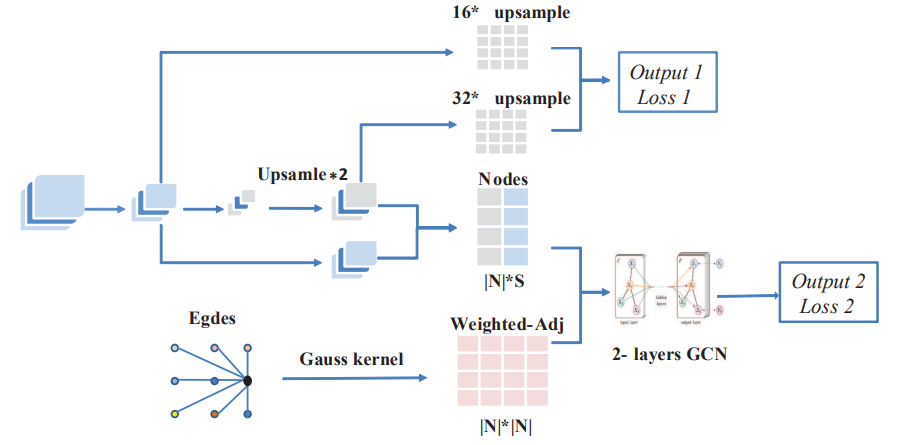
\includegraphics[width=0.8\linewidth]{images/graphfcn_structure.png}
    \caption{Graph-FCN model structure. From ~\cite{lu2020graphfcnimagesemanticsegmentation}.}
    \label{fig:graphfcn_structure}
\end{figure}

\subsubsection{CNN-G}

CNN-G builds on the Graph-FCN model by incorporating a graph-based approach with a convolutional neural network. Two types of structure models are used in CNN-G: distance-based and semantic-based, solved by GCN and GAT, respectively. The distance-based model captures the spatial relationships between nodes, while the semantic-based model focuses on the semantic relationships.

Using a graph attention network (GAT) enables flexible feature extraction across various receptive fields. This approach allows the model to integrate both structure learning and feature extraction.

\textbf{Distance-Based Structure:} Based on the assumption that the closer nodes are more correlated, the Gauss kernel function is used to generate the weighted edges.

The adjacent matrix $A = [e_{ij}]_{|N| \times |N|}$ is used to represent the edge set:

\[
e_{ij} = \begin{cases} \exp \left( -\frac{\|p_i - p_j\|^2}{\sigma^2} \right), & \text{an edge between } n_i \text{ and } n_j \\ 0, & \text{otherwise} \end{cases}.
\]

To simplify the calculation, we make the nodes connect to the $l$ closest nodes.

\textbf{Semantic-based model:} The initial attention coefficient $c_{ij}$ is used to measure the correlation between two nodes. The features of nodes with the same category will be more similar, the attention coefficient between each other will be larger, and the similarity is gradually strengthened in the iteration. A linear transformation is taken to map the concatenation of two nodes' features into a real number: 
\[
c_{ij} = a \left( n_i' || n_j' \right)
\]
The final attention coefficient is obtained through the normalization of all neighborhood nodes: 
\[
e_{ij} = \frac{\exp(c_{ij})}{\sum_{k \in neib_{i}} \exp(c_{ik})}.
\]
When the graph structure is unknown, the matrix $A_{\text{att}} = [e_{ij}]_{|N| \times |N|}$ can be taken as the adjacency matrix. In this case, the edge set is generated by the calculation of the attention coefficients.

In each case, the model generates two outputs, $y1$ and $y2$, which corresponds to two losses, $loss1$ and $loss2$. Both share the convolutional layer's extracted features. The final prediction is based on $y1$. Similar to Graph-FCN, the graph model is only used during training.

The structure of the CNN-G model is shown in Figure~\ref{fig:cnng_structure}.
\begin{figure}
    \centering
    % \fbox{\rule{0pt}{2in} \rule{0.9\linewidth}{0pt}}
    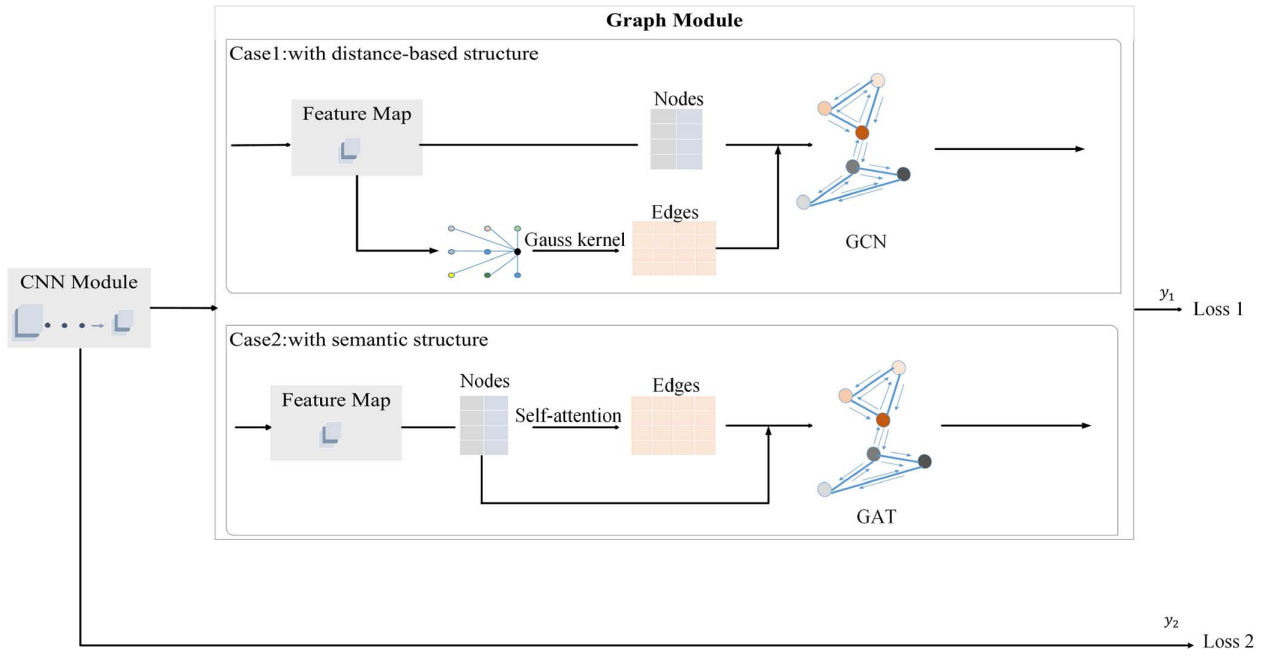
\includegraphics[width=0.8\linewidth]{images/cnng_structure.png}
    \caption{CNN-G model structure. From ~\cite{9103557}.}
    \label{fig:cnng_structure}
\end{figure}

\subsection{Transformer}
\subsubsection{TransUnet}
TransUNet \cite{chen2021transunettransformersmakestrong} has emerged as a robust framework for medical image segmentation by combining the strengths of U-Net and Transformer architectures. Refer the figure \ref{fig:transunet} for the architecture diagram.

\begin{figure}[t]
    \centering
     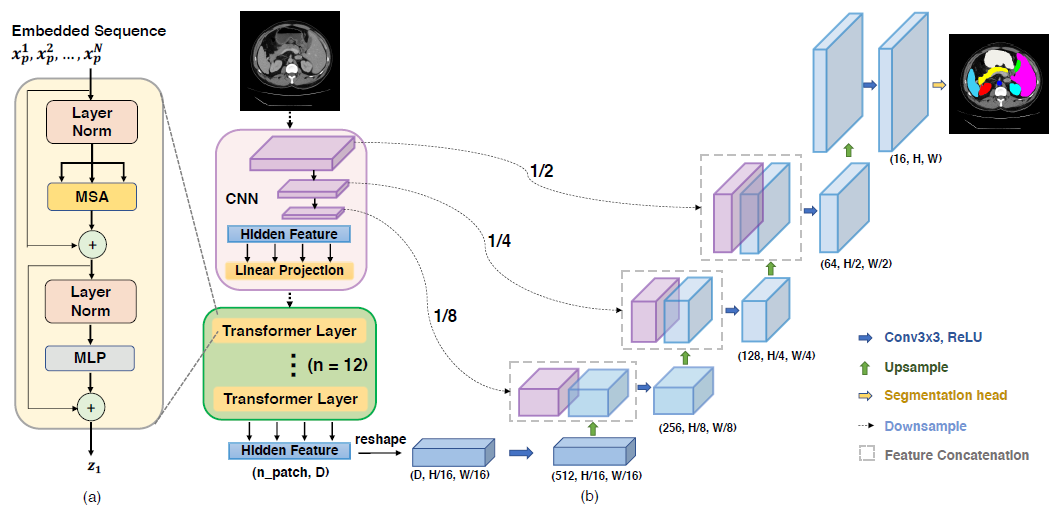
\includegraphics[width=0.9\linewidth]{images/transUnet_arch.png}
  
     \caption{TransUnet architecture. From ~\cite{chen2021transunettransformersmakestrong}.}
     \label{fig:transunet}
\end{figure}

TransUNet addresses these limitations by introducing a hybrid architecture that leverages both CNNs and Transformers. The encoder consists of a CNN followed by a Transformer module. The CNN is used to extract feature maps from the input images, which are then tokenized into image patches and fed into the Transformer. This CNN-Transformer hybrid allows TransUNet to capture detailed spatial features (via CNN) and global context (via the Transformer) simultaneously.

In the decoder, a cascaded upsampling module (CUP) is employed, consisting of multiple upsampling blocks with convolutional layers and ReLU activation. These upsampled features are combined with the high-resolution CNN feature maps from the encoder through skip connections, similar to the U-Net structure, enabling precise localization. This U-Net-like design ensures that TransUNet can recover lost spatial detail while preserving the high-level semantic understanding captured by the Transformer.
\subsubsection{MaskFormer}
Image segmentation models which can solve all 3 tasks (instance, semantic and panoptic segmentation) with a unified architecture started to appear in the literature in the last few years. This started with \underline{DETR} \cite{carion2020endtoendobjectdetectiontransformers} and later improved by \underline{MaskFormer} \cite{cheng2021perpixelclassificationneedsemantic} for semantic segmentation.

\underline{Mask2Former} \cite{cheng2022maskedattentionmasktransformeruniversal}, which adopts the
same meta architecture as MaskFormer, with a backbone, a pixel decoder and a Transformer decoder, extends this to instance segmentation by further improving the neural network architecture in the following ways:
\begin{itemize}
    \item \textbf{Masked Attention}: They use \textit{masked attention} (rather than the standard cross-attention) in the Transformer decoder which restricts the attention to localized features centered around predicted segments, which can be either objects or regions depending on the specific semantic for grouping.
    \item \textbf{Multi-scale high-resolution features}: High-resolution features improve model performance, especially for small objects. However, this is computationally demanding. Therefore, instead of always using the high-resolution feature map, they utilize a feature pyramid which consists of both low and high-resolution features and feed one resolution of the multi-scale feature to one Transformer decoder layer at a time.
\end{itemize}
It also made improvements in optimization and training strategies. The architecture diagram is given in Figure \ref{fig:mask2former}.

\begin{figure}[t]
    \centering
     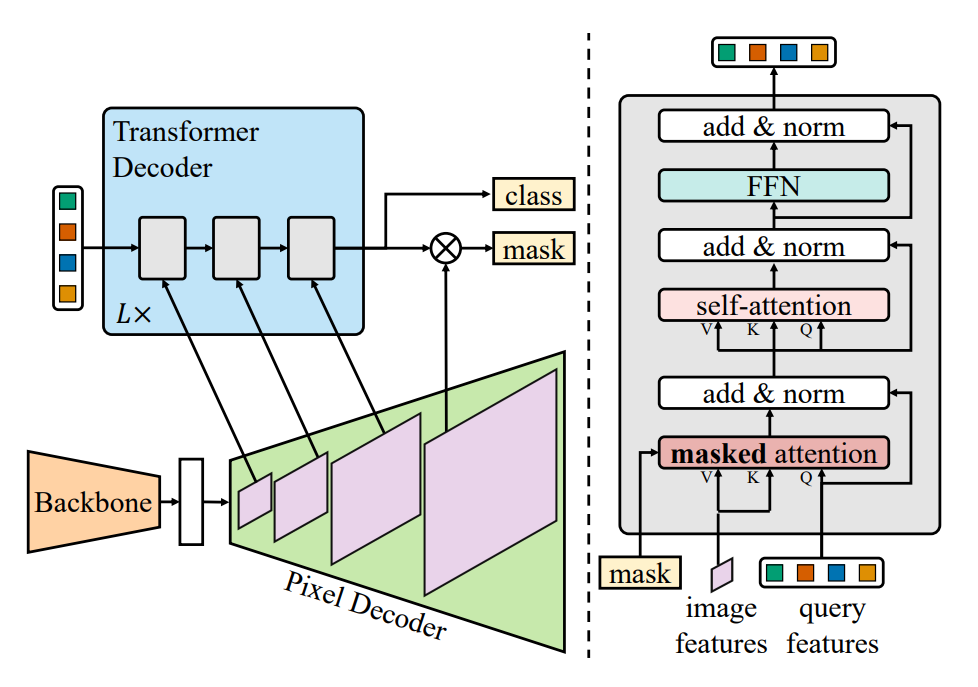
\includegraphics[width=0.8\linewidth]{images/mask2former_arch.png}
  
     \caption{Mask2Former architecture. From ~\cite{cheng2022maskedattentionmasktransformeruniversal}.}
     \label{fig:mask2former}
\end{figure}
\section{Experiments}
\label{sec:experiments}
We conducted an experiment to compare MaskFormer and Mask2Former by fine-tuning them on the Flood-Segmentation dataset \cite{md_faizal_karim_krish_sharma_niyar_r_barman_2022} \textbf{for semantic segmentation}. This dataset consists of 280 RGB images of flood-affected areas, with corresponding ground-truth binary masks (1 stands for flood, 0 for non-flood). Out of the 280 images, we used 200 for training, 20 for validation, and 60 for testing. Out of the 280 images, we used 200 for training, 20 for validation, and 60 for testing.

\subsection{MaskFormer}
To make the fine-tuning more robust, we used the following data augmentation techniques on the training set:
\begin{itemize}
    \item \texttt{Resize}: Randomly resized the images to a size $768\times768$ (ignoring the channel dimension, which is 3).
    \item \texttt{RandomCrop}: Randomly cropped the images to a size $512\times512$.
    \item \texttt{HorizontalFlip}: Randomly flipped the images horizontally with a probability of $0.5$.
    \item \texttt{Normalize}: Normalized each channel of the images with the mean and standard deviation of the pixel values of training set.
\end{itemize}
Note that the spatial transformations (all except \texttt{Normalize}) are applied to the corresponding binary mask.

We used the \textit{facebook/maskformer-swin-base-ade} and \textit{facebook/mask2former-swin-base-ade-semantic} models from Hugging Face's model hub for MaskFormer and Mask2Former, respectively.

\subsubsection*{Fine-tuning}
\textbf{Note:} Since the number of classes were different in the pre-trained model, the classification head was randomly initialized for both the models.

We fine-tuned both of the models for 10 epochs with a batch size of 4. We used the Adam optimizer \cite{kingma2017adammethodstochasticoptimization} with a learning rate of $5\times10^{-5}$ for MaskFormer and $9\times10^{-5}$ for Mask2Former. MaskFormer took around 45 minutes while Mask2Former took around 1 hour to fine-tune on a single Tesla P100-PCIE-16GB GPU.

\subsection{TransUnet}
Transforms perfomed on the training data:
\begin{itemize}
    \item Normalization: Normalized each channel of the images with mean and standard deviation of the training set.
    \item Resize: Resized the images to $256 \times 256$, filling the rest with zeros, keeping the aspect ratio intact.
\end{itemize}

\subsubsection*{Training}
\begin{itemize}
    \item \textbf{Optimizer}: SGD optimizer with a learning rate of $0.01$, momentum of $0.9$, and weight decay of $0.0001$.
    \item \textbf{Loss function}: A combination of Dice loss and cross-entropy loss, with a weight of $0.5$ for each.
    \item \textbf{Epochs}: 150
    \item \textbf{Batch size}: 4
\end{itemize}
On training the TransUnet model, we achieved a mean IoU of $0.9671$ and dice score of $0.98367$ on the validation set, and a mean IoU of $0.96789$ and dice score of $0.98326$ on the test set.
The model was trained on a single single Tesla P100-16GB GPU.
The code is referred from the official implementation of TransUnet \cite{transunet_github}.
\subsection{Graph-FCN \& CNN-G}

Uses DeepLabV3 \cite{deeplabv3} model as the FCN backbone

\paragraph{Training Details}
\begin{itemize}
    \item \textbf{Epochs}: 60
    \item \textbf{Batch Size}: 4
    \item \textbf{Learning Rate}:
    \begin{itemize}
        \item Graph-FCN: $1\text{e-}4$
        \item CNNG: $2\text{e-}5$
    \end{itemize}
    \item \textbf{Optimizer}: Adam
    \item \textbf{Loss}: Cross Entropy
\end{itemize}
\paragraph{MIoU Results}
\begin{itemize}
    \item Graph-FCN: 83.45
    \item CNNG: 84.33
\end{itemize}

\subsection{Experimental Setup for UNet++}

\paragraph{Training Details}
The UNet++ model was configured and trained with the following parameters:
\begin{itemize}
    \item \textbf{Epochs:} 10
    \item \textbf{Learning Rate:} 0.0001
    \item \textbf{Batch Size:} 4
    \item \textbf{Optimizer:} Adam with a learning rate of $1 \times 10^{-4}$
\end{itemize}

\paragraph{Loss Function}
The loss function used was a combination of Binary Cross-Entropy and Dice Coefficient, formulated as:
\[
\mathcal{L}(Y, \hat{Y}) = -\frac{1}{N} \sum_{b=1}^N \left( \frac{1}{2} Y_b \cdot \log \hat{Y}_b + \frac{2 \cdot Y_b \cdot \hat{Y}_b}{Y_b + \hat{Y}_b} \right)
\]
This composite loss function is designed to optimize the model by addressing both class imbalance and the need for precise boundary delineation.

\paragraph{Results}
The UNet++ model achieved the following performance metrics:
\begin{itemize}
    \item \textbf{Best Validation Intersection over Union (IoU):} 0.8291
    \item \textbf{Test IoU:} 0.8032
\end{itemize}

The results demonstrate the effectiveness of UNet++ in segmenting images with high precision, particularly under the constraint of relatively small datasets.
\section{Results}
\label{sec:results}

\subsection{Evaluation Metrics}
\subsection{IoU Score}
Intersection over Union (IoU) is defined as the ratio of the area of intersection between the predicted segmentation map A and the ground truth map B to the area of their union.
\begin{equation*} 
\text{IoU}=  \frac{|A \cap B|}{|A \cup B|}. 
\end{equation*} 

\subsection{Quantitative Comparision}
% table
\begin{table}[h]
    \centering
    \begin{tabular}{|c|c|c|}
        \hline
        Model & mIoU(Val Set) & mIoU(Test Set) \\
        \hline
        UNet++ & 80.32 & 82.91 \\
        Graph-FCN & 83.94 & 83.45 \\
        CNNG & 82.93 & 84.33 \\
        MaskFormer & 88.85 & 86.11 \\
        Mask2Former & 88.70 & 86.16 \\
        TransUnet & 96.71 & 96.89 \\
        \hline
    \end{tabular}
    \caption{Comparison of mIoU scores on validation and test sets}
    \label{tab:results}
\end{table}

% table -> number of parameters
\begin{table}[h]
    \centering
    \begin{tabular}{|c|c|}
        \hline
        Model & Number of Parameters \\
        \hline
        UNet++ & \ 260.8M \\
        Graph-FCN & \ 609.91M \\
        CNNG & \ 609.92M \\
        TransUnet &  105.3M \\
        MaskFormer &  101.8M \\
        Mask2Former &  106.8M \\
        \hline
    \end{tabular}
    \caption{Comparison of number of parameters}
    \label{tab:results}
\end{table}

\subsection{Qualitative Comparision}
The qualitative comparison of segmentation results is shown in Figures \ref{fig:results} and \ref{fig:results2}.
% images
\begin{figure}[t]
    \centering
     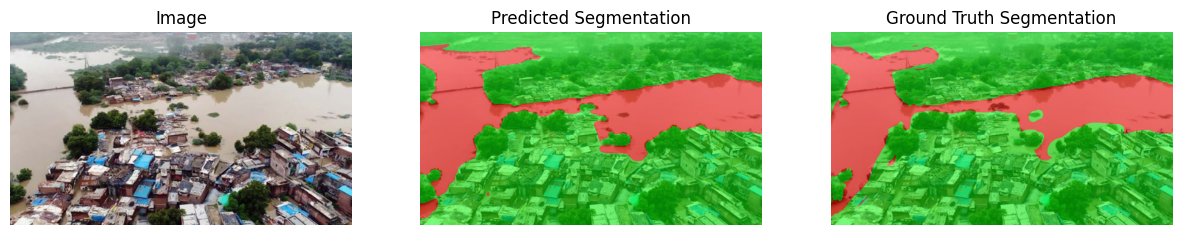
\includegraphics[width=0.9\linewidth]{images/maskformer_1_after.png}
  
     \caption{Qualitative comparison of segmentation results.}
     \label{fig:results}
\end{figure}

\begin{figure}[t]
    \centering
     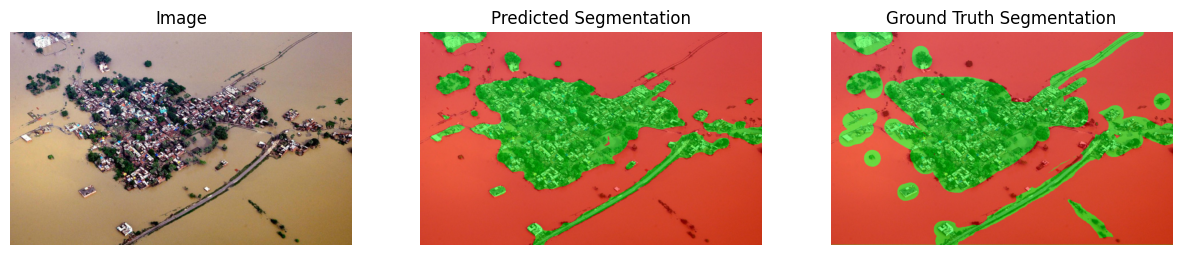
\includegraphics[width=0.9\linewidth]{images/maskformer_2_after.png}
  
     \caption{Qualitative comparison of segmentation results.}
     \label{fig:results2}
\end{figure}
\section{Conclusion}
\begin{itemize}
    \item TransUnet performs the best in terms of \texttt{mIoU} on the validation and test sets.
    \item Even though Mask2Former claim to be better than MaskFormer, it shows only marginal improvement in terms of \texttt{mIoU} on this dataset.
    % \item Interestingly, the absolute value of loss for Mask2Former is much higher as compared to MaskFormer 
    \item Mask2Former (occupies 412M space on disk) has more parameters than MaskFormer (occupies 393M space on disk) which makes it slightly slower for fine-tuning and inference.
    \item CNNG performs better than Graph-FCN which shows the effectiveness of using the GAT network.
\end{itemize}
\section{Code Availability}
\label{sec:code}
The code for the experiments conducted in this study is available at \url{https://github.com/darpan-gaur/dlProject}.
{
    \small
    \bibliographystyle{ieeenat_fullname}
    \bibliography{main}
}

% WARNING: do not forget to delete the supplementary pages from your submission 
% \clearpage
\setcounter{page}{1}
\maketitlesupplementary


\section{Rationale}
\label{sec:rationale}
% 
Having the supplementary compiled together with the main paper means that:
% 
\begin{itemize}
\item The supplementary can back-reference sections of the main paper, for example, we can refer to \cref{sec:intro};
\item The main paper can forward reference sub-sections within the supplementary explicitly (e.g. referring to a particular experiment); 
\item When submitted to arXiv, the supplementary will already included at the end of the paper.
\end{itemize}
% 
To split the supplementary pages from the main paper, you can use \href{https://support.apple.com/en-ca/guide/preview/prvw11793/mac#:~:text=Delete%20a%20page%20from%20a,or%20choose%20Edit%20%3E%20Delete).}{Preview (on macOS)}, \href{https://www.adobe.com/acrobat/how-to/delete-pages-from-pdf.html#:~:text=Choose%20%E2%80%9CTools%E2%80%9D%20%3E%20%E2%80%9COrganize,or%20pages%20from%20the%20file.}{Adobe Acrobat} (on all OSs), as well as \href{https://superuser.com/questions/517986/is-it-possible-to-delete-some-pages-of-a-pdf-document}{command line tools}.

\end{document}
